%% Use the option review to obtain double line spacing
%% \documentclass[authoryear,preprint,review,12pt]{elsarticle}

%% Use the options 1p,twocolumn; 3p; 3p,twocolumn; 5p; or 5p,twocolumn
%% for a journal layout:
%% \documentclass[final,1p,times,authoryear]{elsarticle}
%% \documentclass[final,1p,times,twocolumn,authoryear]{elsarticle}
%% \documentclass[final,3p,times,authoryear]{elsarticle}
%% \documentclass[final,3p,times,twocolumn,authoryear]{elsarticle}
%% \documentclass[final,5p,times,authoryear]{elsarticle}
\documentclass[final,5p,authoryear]{elsarticle}
%% For including figures, graphicx.sty has been loaded in
%% elsarticle.cls. If you prefer to use the old commands
\usepackage{amssymb}
%% The amsthm package provides extended theorem environments
%% \usepackage{amsthm}
\usepackage{lineno}
\usepackage{booktabs}
% ---------------------------------------------------------------------
%             FOR DRAFTING / REVIEW (DELETE BEFORE SUBMISSION)
% ---------------------------------------------------------------------
\usepackage{caption}
\usepackage{subcaption}
\usepackage[T1]{fontenc}
\usepackage[british]{babel}
\usepackage{microtype}
\usepackage[tt=false]{libertine}
\usepackage{xcolor}
\definecolor{blue}{RGB}{33,150,209}
\definecolor{red}{RGB}{255,0,0}
\usepackage{xurl}
\usepackage[colorlinks=true, allcolors=blue]{hyperref}
\usepackage{pdfpages}
\usepackage{enumitem}
\usepackage{lineno}
\usepackage{float}
\setlength{\linenumbersep}{5pt}
% Save the old \texttt command
\let\oldtexttt\texttt
% Redefine the \UrlFont to use a smaller typewriter font
\renewcommand{\UrlFont}{\ttfamily\small}
% Redefine the \texttt command to use a smaller font size and allow line breaks
\renewcommand{\texttt}[1]{{\ttfamily\small\nolinkurl{#1}}}

\usepackage{tcolorbox}
\newcommand{\cbox}[1]{
    \begin{tcolorbox}[hbox, colback=red!5!white, colframe=red!65!black, boxrule=0.25pt, boxsep=2pt, left=2pt, right=2pt, top=1pt, bottom=1pt]
        \small\sffamily #1
    \end{tcolorbox}
}

% ------------------------------------------------------

\journal{Resources, Conservation and Recycling}

\begin{document}


\linenumbers

    % SPOTLIGHTS (5 bullet points, max 120 characters each)
    {\Large Spotlights}
    \vspace{1em}
    \begin{description}[style=nextline]
        \item[Bullet 1: Critical context and background information on the problem addressed] Tracking waste and material flows is essential for developing the circular economy and supply chain resilience
        \item[Bullet 2: A brief overview of the key finding of the study (or findings if necessary)] A tool was developed to quantify waste and material footprints of activities in life cycle assessment (LCA) databases
        \item[Bullet 3: The most radical, creative, disruptive or innovative aspect of the manuscript] Built to complement the Brightway LCA framework and ActivityBrowser, the tool is customisable and easy to use.
        \item[Bullet 4: The significance of the results to the environment, economics or society] The tool can be used to identify pre-consumer waste and material hotspots that are often hidden in supply chains.
        \item[Bullet 5: Future vision or the most important implications for continued research] Improved data availability and quality would enable more detailed and accurate waste and material footprinting.
    \end{description}

    \newpage
    %% GRAPHICAL ABSTRACT
    \begin{graphicalabstract}
        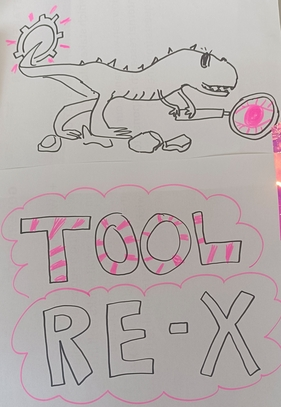
\includegraphics{grabs}
    \end{graphicalabstract}

    %% RESEARCH HIGHLIGHTS (3-5 bullet points, max 85 characters each)
    \begin{highlights}
        \item T-reX, a new tool for quantifying waste and material flows in LCA.
        \item Assesses supply risks by calculating demand for critical materials.
        \item Simplifies quantification of user-specified waste and material categories.
        \item Rapidly identifies waste and material demand hotspots.
        \item Presents a case study of the battery supply chain.
    \end{highlights}


\begin{frontmatter}

    \title{T-reX: A python package to quantify supply chain flows of waste and material in LCA databases}
    \author[1]{Stewart Charles McDowall\corref{cor1}}
    \ead{s.c.mcdowall@cml.leidenuniv.nl}
    \author[1]{Elizabeth Lanphear}
    \author[1]{Stefano Cucurachi}
    \author[1]{Carlos Felipe Blanco}

    \cortext[cor1]{Corresponding author:}

    \affiliation[1]{
        organization={Institute of Environmental Sciences (CML), Leiden University},
        addressline={P.O. Box 9518},
        city={Leiden},
        postcode={2300 RA},
        state={South Holland},
        country={The Netherlands}}

    \begin{abstract}
        \cbox{Abstract word count: 164, Limit: 150}
        Minimising waste through the reuse of resources is the quintessential principle of the `circular economy', but relies on our ability to identify and quantify waste and material flows.
        Thus, identifying and quantifying waste and material flows are of fundamental importance. Life Cycle Assessment (LCA) is powerful for this end, given its capacity to pinpoint hotspots of environmental impact throughout the life cycle of products and services, those where the implementation of circular principles could be most effective.

        Introducing T-reX, a Python tool extending the Brightway framework for flexible quantification of user-defined supply-chain demands in current and future scenarios. This tool streamlines database manipulation for LCA practitioners and integrates methods to aggregate and analyse waste and material flows, facilitating rapid hotspot identification.

        A case study on battery supply chains demonstrates the tool's utility. T-reX quantifies and compares inventory demands and, thus, potential environmental burdens, aiding sustainable decision-making. It contributes to the development of the `circular economy' by providing detailed material usage and waste generation analysis.

    \end{abstract}


    % KEYWORDS (max 6)
    \begin{keyword}
        circular economy \sep waste \sep material \sep life cycle assessment \sep critical raw material \sep supply chain
    \end{keyword}

\end{frontmatter}
\cbox{Total word count: ~6000, Limit: 5000 (can be easily condensed)}

%% main text
\section{Introduction}
\label{sec:introduction}
\cbox{Section word count: 1450}
\cbox{To be split into two (sub) sections: Introduction and Background, can be easily condensed by 200 words or so.}
The development of a `circular economy' has become a critical area of focus in the imperative pursuit of achieving sustainability objectives and curtailing our environmental footprint within planetary boundaries~\citep{eu2019greendeal, eu2020circ,nl2023ceplan,nl2016ceplan,pardo2018ce,ellenmacarthur2015ce}. Fundamental to this development is a decrease in primary material consumption and a reduction of life cycle waste through the implementation of `re-X' strategies (e.g., refuse, rethink, design for---and implementation of---repair, remanufacturing and recycling)~\citep{eu2022ecodesign, eu2022repair,eu2015reman}. In addition to circular economy goals, contemporary geo-political tensions in an ever more globalised economy have highlighted the vulnerability of many advanced economies to intentional supply disruptions, wrought as an act of competition or outright hostility~\citep{jrc2023supplychain,hartley2024cepolitics,berry2023crm}.

While some material demands are apparent in the final product and the waste generated may be inferred from knowledge of the use-- and end-of-life-- (EOL) phases, a significant proportion of these are often `hidden' in the supply chain and thus not reported directly in the final results~\citep{laurenti2016wastefootprint,salviulo2021supplychain}. It has been found that these material footprints can be `highly representative of damage to human health and biodiversity'~\citep{steinmann2017resourcefootprints} and that waste footprints have a `strong association' with environmental damage~\citep{laurenti2023wastefootprint}. Thus, to reduce the negative externalities of consumption and improve supply chain resilience, it is essential to uncover, disaggregate, and quantify the material and waste footprints of human activities in as much detail as possible.


Life Cycle Assessment (LCA) is a useful method for the holistic estimation of the environmental impacts of products and processes. LCA can comprehensively evaluate these impacts across the entire life cycle---from `cradle to grave'---, often identifying critical hotspots and guiding prioritisation of actions. The standard approach is to apply Life Cycle Impact Assessment (LCIA) methods (such as ReCiPe~\citep{huijbregts2016recipe} and CML~\citep{guinee2002cml}), which convert the inventory data into a set of impact scores based on the sum of the elementary flows. These scores are then aggregated into a single score for each impact category, which can be compared across products and processes.

Several LCIA methods include, to some extent, waste generation~\citep{foen2021ecofactors,hauschild2003edip,cen2019en15804} and material consumption~\citep{arvidsson2020csi,foen2021ecofactors}. These methods, however, are generally limited in their scope (especially for waste), do not allow for flexible quantification of specific waste and material types, and often provide results in characterised units that are abstract or difficult to interpret (e.g., Ümweltbelastungspunkte (UBP)).


In the context of a mineral-hungry renewable energy transition and recent geo-political tensions, more attention is being paid to the security of supply of materials, especially those considered `critical raw materials' (CRMs)~\citep{eu2023crmstudy,hool2023crm,mancini2013supplysecurity,jrc2023supplychain,hartley2024cepolitics,salviulo2021supplychain}. While LCA seeks to model the technosphere (a.k.a. the anthroposphere), its focus is often on the environmental impacts of the system---the endpoints--- rather than the primary material flows themselves. 

A relatively new method, termed the crustal scarcity indicator (CSI)~\citep{arvidsson2020csi}, was developed to assess long-term global scarcity of minerals in LCA. This method introduced crustal scarcity potentials (CSPs) measured in kg silicon equivalents per kg element, derived from crustal concentrations. CSPs, provided for 76 elements, reflect the long-term global elemental scarcity based on crustal concentration proxies. The CSI, calculated by multiplying CSPs with extracted masses, effectively gauges the impact of elemental extraction. 

While useful for its stated purpose, the CSI presents its midpoint results in an abstract unit (kg-Si eq.) that is difficult to interpret and compare with other impact categories. Furthermore, the CSPs are not available for all elements (or more complex materials), and the method does not allow for the quantification of material demands in terms of mass or volume.


\subsection{Waste in LCA}

Though often described simply as a `material with a negative economic value'~\citep{guinee2004economicallocation}, waste is a nebulous concept, and one whose definition is poorly delineated and variable across space and time.  Moreover, from a systems perspective, the notion of waste is anathema to the circular economy, and it is far more useful to consider the identity and nature of the specific material flows. Thus, precise and detailed categorisation of these is essential to understand the `circularity' of an activity and its life cycle externalities. There is a conspicuous gap in the understanding of the waste footprint of human activities and their relationship with environmental damage~\citep{laurenti2023wastefootprint}. Conventional LCAs consider waste as a `service'~\citep{guinee2021wasteisnotaservice} and typically use generic waste processing models~\citep{beylot2018} that break the causal link between the functional unit and the waste-associated impacts.

In LCA, waste flows are not considered as fundamental biosphere exchanges, but rather as technosphere flows. Waste produced by an activity is transferred to a relevant waste treatment activity where it is accepted `burden-free' and transformed into a combination of emissions and other waste `products'~\citep{guinee2021wasteisnotaservice}. There can be several treatment steps in this pathway leading, ultimately, to a mass of material being deposited in a landfill. In this system of waste accounting, the impacts apportioned to the waste-producing activity are a sum of those incurred by the transport, treatment, and final disposal of the waste into terrestrial or aquatic environments. In particular, the extensive work of~\cite{doka2024publications} has contributed significantly to understanding the environmental impacts of waste treatment processes and the long-term impacts of disposal.

A significant portion of a product's total waste is generated during earlier stages such as resource extraction, transportation, and manufacturing, often remaining `invisible' in traditional LCA practices~\citep{laurenti2016wastefootprint}. This oversight in measuring and communicating a cradle-to-grave product waste footprint (PWF) highlights a gap in circular economy indicators. Traditional LCA does not typically view waste as having environmental significance by itself, focusing instead on emissions and resource use resulting from waste treatment. The environmental significance of waste and its correlation with other indicators has been the subject of extensive research. For example, studies have shown that popular resource footprints can cover a significant portion of environmental impact variance in product rankings~\citep{steinmann2017resourcefootprints}. However, correlations between various environmental indicators are not always consistent, as seen with the carbon footprint, which often does not correlate with other impact assessment scores~\citep{laurent2012carbonfootprint}. The aggregation of waste in PWFs raises concerns among LCA experts, regarding the uncertainties introduced by aggregated measures, as well as the potential misrepresentation of environmental performance due to differences in waste types~\citep{chen2021methoduncertainty,huijbregts2010energyfootprint}.

Moreover, existing LCA methodologies offer limited direct indicators at the impact assessment level, providing sparse information on the impacts of waste. This limitation becomes particularly evident when attempting to identify waste generation hotspots within a product's life cycle. Addressing these hotspots is crucial for advancing towards circularity, however,  there is a lack of a convenient and flexible way to calculate waste flows in LCA and a pressing need for more comprehensive methods that can effectively quantify waste flows and, therefore, contribute to a better understanding of a product's total environmental footprint.
\cite{laurenti2023wastefootprint} developed a method to calculate the waste footprint of a product or service based on solving the demand vectors of the activities, also presenting simple measures to quantify waste hazardousness and circularity. In that study, it was shown that the waste footprint correlates well with other LCIA methods, particularly human health. The method presented, however, is limited in its scope and flexibility, is computationally intensive, difficult to use, is not easily reproducible, and suffers from errors due to double counting. The T-reX tool presented herein provides a more flexible, transparent, and user-friendly approach to quantifying waste flows in LCA. Moreover, the T-reX tool is not limited to waste but can be used to quantify any supply-chain flow, such as water, gas, and critical raw materials. 

\subsection{The T-reX Tool}

To better assess waste and material flows in LCA, we have developed a Python program built on the Brightway framework~\citep{mutel2017brightway} and designed to track these exchanges by translating them into indicators and `pseudo' LCA impact (LCIA) categories. In this study, we present the T-reX tool that enables LCA practitioners to manipulate their databases to allow them to easily aggregate the mass and volume of any desired exchange, and to create flexible categories that differentiate between material categories, waste types, and EOL handling.

While methods with similar aims exist, they lack customisability and specificity~\citep{foen2021ecofactors} or can be cumbersome to apply and suffer from errors due to multiple counting~\citep{laurenti2023wastefootprint}.

The purpose of the T-reX tool is not to quantify the environmental impacts of material consumption and waste production, but rather to quantify the material and waste flows themselves, even those that are finally consumed by waste treatment processes. It provides, thus, not an impact assessment in the traditional sense, but an accounting of the material consumed and waste generated by a product or service inside of the technosphere, regardless of the end-of-life fate of these flows. By definition, the development of the `circular economy' necessitates the reduction and ultimate elimination of waste---though whether this objective is thermodynamically impossible has long been the subject of debate by~\cite{ayres1998recycling},~\cite{reuter2012recyclinglimits} and many others. In any case, avoiding material consumption and generation of waste is of paramount importance. By allowing LCA practitioners to easily classify and quantify these exchanges, the T-reX tool provides a practical means to identify hotspots and opportunities for waste reduction and material efficiency.






\section{Methodology}
\label{sec:methodology}
\cbox{Section word count: 2000}
This section is divided into two parts. In \autoref{sec:method-TreX}, we describe the T-reX program, and in \autoref{sec:method-casestudy}, we describe the methodology used to calculate the waste and material inventory footprints in a case study of five Li-ion batteries.

\subsection{T-reX}\label{sec:method-TreX}

\subsubsection{Computational framework}

Developed in the Python programming language, T-reX extends the \texttt{brightway LCA framework}, utilising the components \texttt{bw2data}, \texttt{bw2calc}, and \texttt{bw2io}~\citep{mutel2017brightway}. Additionally, the \texttt{wurst} package---which can deconstruct databases into a list of exchanges---is used to facilitate searching and data transformation at the exchange level (the individual supply chain flows)~\citep{mutel2017wurst}. Integration with the \texttt{premise} package~\citep{sacchi2022premise}---which integrates the projections of integrated assessment models (IAMs) into current LCA databases---enables the user to easily create and manipulate prospective LCA databases. T-reX is also compatible with \texttt{ActivityBrowser}~\citep{steubing2020activitybrowser}---an open-source graphical user interface for LCA---and after running T-reX, the manipulated databases and the `pseudo-LCIA' methods created by T-reX can be used in the project in the accustomed way. T-reX is installable via the Python Package Index (PyPI)~\citep{mcdowall2023T-reXpipy} and is fully open-source under the CC-0 licence. The full source code for T-reX is indexed on Zenodo~\citep{mcdowall2023T-reXzenodo} and under further development in the GitHub repository~\citep{mcdowall2024T-reXgithub}. T-reX is designed to be used with \texttt{ecoinvent} databases~\citep{ecoinvent2016version3}, but could be adapted to other databases by changing the search criteria. Currently, it has been tested with all available system models of \texttt{ecoinvent}versions 3.5--3.10.

T-reX can be used directly from the command line, or imported as a Python package where the user can access the individual functions and modules. In the simplest case, the user can run the program with the default settings, which will calculate the waste and material footprint of the \texttt{ecoinvent}database. The user can adapt the settings of T-reX as desired, to calculate alternative or additional waste and material inventory footprints, use a custom database, or a `prospective' database based on future scenarios by implementing the premise \texttt{premise} with one of T-reX's internal modules.

The supplementary material in \autoref{sec:supplementary} contains metadata of T-reX, along with a list of the constituent modules, a description of their functions, and a detailed computational workflow. Further details can be found in the GitHub repository and package documentation~\citep{mcdowall2024T-reXgithub, mcdowall2023T-reXdocs}.

\subsubsection{Functionality and purpose}

T-reX is a Python package that enables one to produce LCA databases---both current and prospective---that are manipulated to facilitate the calculation of waste and material inventory footprints in the supply chain of any activity in the same way as one would apply standard LCIA methods. We refer to the T-reX methods as `pseudo-LCIA' methods, as they represent an accounting of an activity's technosphere inventory without reference to impact modelling, as in standard LCIA.

If desired, prospective databases can be defined by the user or constructed with the projections of the integrated assessment models such as IMAGE~\citep{stehfest2014image} and REMIND~\citep{remind2020model}, which offer a range of options aligned with the Shared Socioeconomic Pathways (SSPs)~\citep{ssp2020ghg} and can be paired with a variety of mitigation scenarios.

The deconstruction of the databases by T-reX into lists of exchanges allows the relevant flows of material and waste to be identified and categorised by the search functions. The queries facilitating this are tailored to the specific database and the user can easily modify them to suit their needs. The categories defined in the configuration are used to create T-reX's `pseudo LCIA' methods that are indicators of aggregated technosphere demand. The exchange editing function of T-reX then takes each list of exchanges and appends to the relevant activity a copy of the technosphere exchange as a mirrored `pseudo-biosphere' exchange that matches the `pseudo-LCIA' method.

In the default configuration, there are 10 waste categories which are further divided by their unit of measurement (kilograms and cubic meters) to create a total of 20 waste methods. The waste categories include incineration, recycling, and total waste, and are listed in the supplementary material in~\autoref{sec:supplementary}. One advantage of T-reX is that it can identify `hidden' waste exchanges that would otherwise be `consumed' by a treatment process and not leave the technosphere. Since `waste is not a service'~\citep{guinee2021wasteisnotaservice}, a characterisation factor of -1 is applied to the waste footprint methods (except CCS exchanges), changing the perspective from `waste consumed by treatment' to `waste generated by the activity'.

In addition to the waste categories, T-reX can incorporate any number of material demand categories, the defaults being based on the EU Critical Raw Materials (CRM) list for 2023~\citep{eu2023crmstudy}, which contains 30 materials considered essential to the EU economy and also at risk of supply disruption. Especially valuable in the case of CRMs is T-reX's ability to uncover and quantify these threads of background consumption, which can be inconspicuously embedded in products or consumed in seemingly distant supply chain activities. The identity of the materials considered and their categorical groupings are easily customisable by the user, and in further materials of interest to the authors were added to the example Li-ion case study, including helium, electricity, petroleum, sand, water, and natural gas. The full list of 59 materials included in the default configuration is provided in the supplementary material in ~\autoref{sec:supplementary}.

The logic for the identification of material exchanges with T-reX differs from that used to identify waste exchanges in that the search queries are based on the names of the relevant `market activities' for the material of interest rather than keywords in the exchange's name. A useful feature of T-reX is that, in cases where there are several markets for one material or material group, the program can aggregate these flows. For example, exchanges with markets for the rare-earth-elements (REEs) `market for cerium', `market for dysprosium', `market for erbium', etc.\ can be aggregated into a single indicator category for REEs. Similarly, the total demand for all critical raw materials (CRMs) can be calculated in the same manner.

% As presented in~\autoref{sec:intro-background},~\autoref{sec:intro-waste}, and~\autoref{sec:intro-material} of the introduction, there are some existing material demand methods in the standard LCIA method sets, including the CSI (which provides only an aggregated, abstracted endpoint in units of kg~Si~eq)~\citep{arvidsson2020csi} and the (deprecated) EDIP 2003 material use indicators (which provide endpoints in fundamental units)~\citep{hauschild2003edip}.

In these methods, the material demand is calculated based on the total mass that is extracted from the environment, thus, their focus is essentially solely on the mining-related exchanges that bring these materials from the biosphere into the technosphere.

T-reX, in contrast, uses accounting for material demand and waste generation based on exchanges solely within the technosphere. This offers a different perspective, allowing for the estimation of overall supply chain material demands that consider the entire life cycle of an activity, including non-direct impacts on the market such as co-production of other materials. Consider a demand for an activity containing a metal, for example; while the existing material use methods allow one to calculate the total mass of that metal that is extracted from the environment, T-reX can provide insight into the broader supply chain impacts of the demand for this metal. If the production of other materials is attributed to the production of this metal, these would appear as negative material demands in the T-reX results---supply chain pressure for one material can result in lessening of supply chain pressure for another. In the results of the Li-ion battery case study in \autoref{sec:results-casestudy}, we will see that this is indeed the case for nickel demand, which, in the final inventory because of such co-production, is counter-intuitively negative (due to co-production and substitution in the LCA system models) despite the presence of nickel in the final products.

% \subsubsection{Mathematical basis}

% \cbox{very nice formulae coming soon from LL hopefully}

\subsubsection{The workflow of T-reX}

The workflow of T-reX is divided into several modules, each performing a separate function. The modules are designed to be used in a particular order, but the user can also use them individually to perform specific tasks. The standard workflow is as follows:

\begin{enumerate}
    \item Configuration of waste and material exchange categorisation (optional)
    \item Generation of prospective LCA databases (optional)
    \item Database expansion---to create a list of all exchanges in the database
    \item Identification and categorisation of exchanges
    \item Creation of `pseudo-biosphere' databases
    \item Creation of `pseudo-LCIA' methods to calculate waste and material inventory footprints
    \item Exchange editing---whereby the technosphere exchange is mirrored as a `pseudo-biosphere' exchange
    \item Database verification---to ensure that T-reX has manipulated the database correctly
\end{enumerate}

This workflow creates a copy of the original \texttt{brightway} project containing the original biosphere database, a T-reX `pseudo-biosphere' database along with one or more manipulated technosphere databases that can be used to calculate the waste and material inventory footprints of activities in the same way as standard LCIA calculations.

An overview of the T-reX workflow is presented in \autoref{fig:methods-flowchart}. The supplementary material in \autoref{sec:supplementary} contains a more detailed computational flowchart.

\begin{figure}[H]
    \centering
    \caption{Workflow of T-reX. Application of T-reX to one or more LCA databases creates a \texttt{brightway} project with customised methods and activities that can be used to calculate waste and material inventory footprints of the activity's supply chain.}
    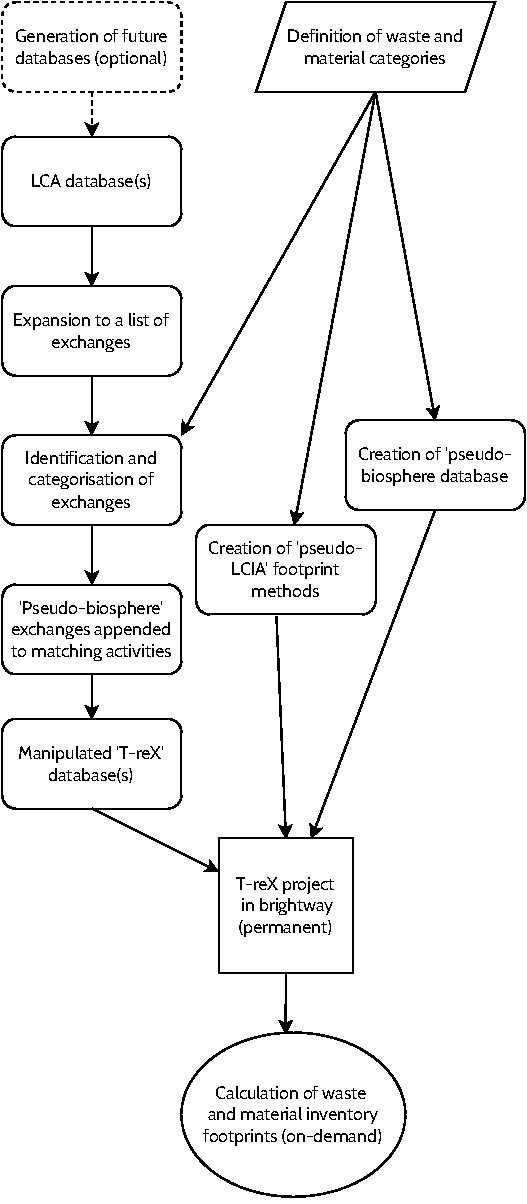
\includegraphics[width=14cm]{figures/T-reX_method.pdf}\label{fig:methods-flowchart}
\end{figure}


\subsection{Case study methodology}\label{sec:method-casestudy}

We investigated five types of Li-ion batteries, each represented by their unamended global market activities:
\begin{itemize}[itemsep=0pt]
    \item Li-ion, LFP, rechargeable, prismatic
    \item Li-ion, LiMn\(_2\)O\(_4\), rechargeable, prismatic
    \item Li-ion, NMC111, rechargeable, prismatic
    \item Li-ion, NMC811, rechargeable, prismatic
    \item Li-ion, NCA, rechargeable, prismatic
\end{itemize}

In addition to the waste and material inventory footprint methods created by T-reX, the following standard LCIA methods were applied for comparison:

\begin{itemize}[itemsep=0pt]
    \item ReCiPe 2016 v1.03, midpoint (I)
    \item EF v3.0 no LT
    \item EDIP 2003 no LT
    \item CSI 2020
\end{itemize}

The source of the life cycle inventory data for this case study was \texttt{ecoinvent}, version 3.9.1, with the `cutoff' attributional system model. Additionally, T-reX was used to create prospective database sets using the functionality of \texttt{premise} with the REMIND model and the baseline scenario SSP2 `middle of the road' with the following Representative Concentration Pathways (RCPs):
\begin{itemize}
    \item SSP2-base: representing an approximate 3.5°C increase in global temperatures to 2100
    \item SSP2-PkBudg500: representing the achievement of Paris climate goals, ca. 1.3°C increase to 2100
\end{itemize}

For each pathway, databases (at five-year time intervals) were created with \texttt{premise}~\citep{sacchi2022premise} and processed with T-reX for the period between 2020 and 2100.

\subsubsection{LCA calculations}
For each combination of activity, method, and database, a single score was calculated along with details of the top contributing processes. Additionally, for the T-reX methods, a contribution analysis was performed. This involved utilising the \texttt{bwa.compare\_activities\_by\_grouped\_leaves} function from the \texttt{brightway2\_analyzer} package~\citep{mutel2016brightway2analyzer}, a component of the \texttt{brightway} ecosystem. This function performs graph traversal on the impact matrix of the LCA object to a specified cutoff and groups the resulting leaves by their Cooperative Patent Classification (CPC) codes. This provides insight into the products and sectors in the supply chain of the activity that carry the most substantial responsibility for the final waste generation or material demand footprints.




\section{Results}
\cbox{Section word count: 1400}
\label{sec:results}
\subsection{T-reX tool}\label{sec:results-T-reX}

An example of the output from the application of T-reX has been included in the supplementary material in~\autoref{sec:supplementary}. The manipulated \texttt{ecoinvent} databases (which are the main product of T-reX) can be recreated by following the instructions in the package documentation~\citep{mcdowall2023T-reXdocs}.

\subsection{Case study: Li-ion batteries}\label{sec:results-casestudy}

As described in~\autoref{sec:method-casestudy}, this case study calculated the waste and material footprints (with a variety of other indicators) for the unaltered background inventories of five Li-ion batteries with the functional unit being 1~kg of the battery at the global market. The purpose of this simple case study was to test, verify, and demonstrate the functionality and limitations of T-reX. This section includes some highlights of the results, with full results included in the supplementary material (\autoref{sec:supplementary}). Because the `pseudo-LCIA' methods created by T-reX are integrated into the user's \texttt{brightway} project as if they were standard LCIA methods, the footprint calculations can be performed in the customary way. In the supplementary material, there are screenshots of selected results obtained using the \texttt{ActivityBrowser} software, including contribution analysis and a Sankey diagram that disaggregates the final footprint result over the activities in the supply chain.

\subsubsection{Sankey visualisation of flows in waste and material inventory footprints}\label{sec:results-case_study-sankey}

\autoref{fig:sankey_waste} presents a Sankey diagram depicting the supply chain flows of `total solid waste' attributed to the NMC 811 Li-ion battery at the global market in the \texttt{ecoinvent} database version 3.9.1. As the supply chains are expansive, this visualisation has been greatly simplified for print, the full version is included in the supplementary material~\autoref{sec:supplementary}. As is evident in the figure, the largest contributors to the waste footprint are the extraction and processing of the raw materials, with the largest flows coming from the extraction of cobalt, lithium, and nickel. Due to the nature of LCA, the waste flows do not represent the `real' physical flows directly, but rather an abstraction thereof based on, in this case, economic allocation---the market price of the functional unit produced by the activity~\citep{guinee2004economicallocation}. If an unallocated database were available, the waste flows could be calculated with T-reX in the same way and be more directly related to the physical flows of the activities.

\begin{figure}[H]
    \centering
    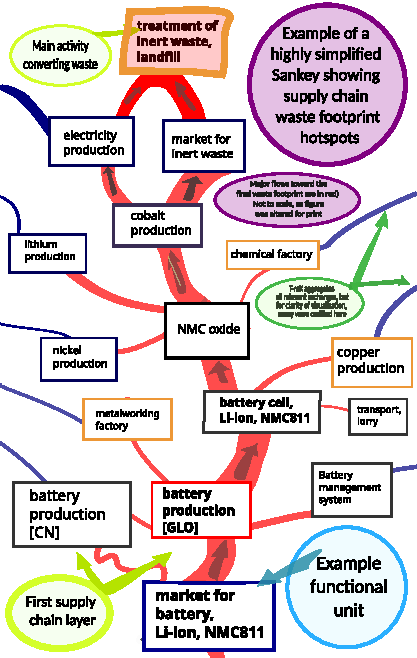
\includegraphics[width=8cm]{figures/T-reX_NMC811_WasteTotalSolid.pdf}
    \caption{A simplified Sankey diagram from \texttt{ActivityBrowser} showing the total solid waste footprint flows for the NMC 811 battery supply chain at the global market in the \texttt{ecoinvent} database version 3.9.1.}\label{fig:sankey_waste}
\end{figure}

\subsubsection{Temporal and scenario variation in waste and material inventory footprints}
%\label{sec:results-case_study-total_footprints}

%! total
\autoref{fig:waste_totalANDcarbon} (a) shows the `total solid waste' inventory footprint for the five Li-ion batteries in the case study from 2020 to 2100 under the SSP2 scenario using the baseline and PkBudg500 RCPs of the REMIND model. The NMC811 battery has the largest footprint, producing over 50~kg of waste per kilogram of battery produced. The  LiMn\(_2\)O\(_4\) battery has the smallest footprint, producing less than 4~kg of waste per kilogram of battery. In each case, there was only a slight downward trend in the waste footprints between 2020 and 2100. This is mostly in the period between 2020 and 2040 and could be attributable to the relatively rapid decrease in fossil fuel use that is factored into the models over this time (since many produce relatively large amounts of waste during extraction and combustion). For the total waste generated by these batteries, there was very little difference observed between the baseline and PkBudg500 RCPs.

%! CO2
The inclusion of carbon capture and storage (CCS) in the prospective databases is apparent in~\autoref{fig:waste_totalANDcarbon} (b), with the rapid increase in the production of carbon dioxide `waste' over the period from 2020--2040 that is not seen in the baseline scenario. This result highlights the fact that the (often) downward trends in global warming impacts calculated with prospective databases using standard LCIA methods are dependent on the assumptions made about the introduction of CCS technology. The actual deployment of these technologies was only around 37~Mt CO$_2$/yr as of 2023~\citep{dziejarski2023ccs}, far short of the levels projected in many of the RCP scenarios~\citep{sacchi2023premisedocs}. The authors consider that the over-representation of CCS and the under-representation of waste processing technologies in the prospective databases is one significant limitation to the validity of prospective LCA databases. Significant work is needed to improve the representation of these technologies in the databases to ensure that the results are more realistic and useful for decision-making.
%!!!!

\begin{figure}[H]
    \centering
    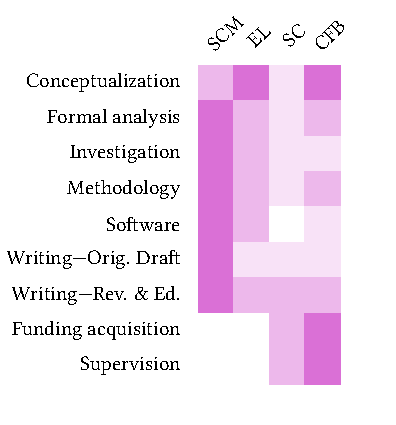
\includegraphics[width=16cm]{figures/T-reX-wastefootprint-totalANDcarbon.pdf}
    \caption{T-reX calculated supply chain inventories for the five Li-ion batteries in the case study, showing their `footprints' for: (a) total solid waste, and (b) carbon dioxide waste (from carbon capture and storage (CCS) only). The footprints were modelled with prospective LCA databases from 2020 to 2100 under the SSP2 scenario using the baseline and PkBudg500 RCPs of the REMIND model.}\label{fig:waste_totalANDcarbon}
\end{figure}
%!!!!

\subsubsection{Contribution of `top-processes' in the supply chain}%\label{sec:results-case_study-topprocesses}

\autoref{fig:top_contribution} shows the contribution of the `top-processes' to the graphite footprint of the  LiMn\(_2\)O\(_4\) battery under the baseline scenario from 2020--2100. The total footprint is seen to more than triple, from 0.16~kg/kg in 2020 to 0.52~kg/kg in 2050 and onward to 2100. The largest contributor is not, in this case, the battery-embedded graphite electrode (which is the second top process), but `silicon production' from further up in the supply chain. This result is likely a reflection of the electrification of the transport and energy sectors that is included in the REMIND model. The results of this kind of analysis with T-reX can be used to identify the most significant processes in the supply chain and to target interventions to reduce the potential environmental impact of production.

\begin{figure}[H]
    \centering
    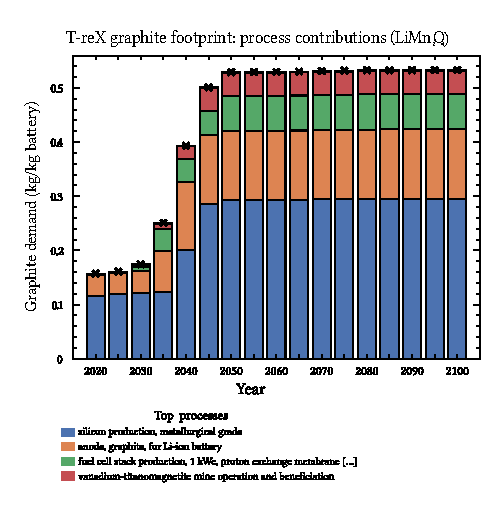
\includegraphics[width=9cm]{figures/T-reX-wastefootprint-processcontributions.pdf}
    \caption{Contribution by the `top-processes' to graphite demand inventory of the LiMn\(_2\)O\(_4\) battery from 2020 to 2100 under the SSP2 scenario using the baseline RCPs of the REMIND model.}\label{fig:top_contribution}
\end{figure}

%!!!!

\subsubsection{Contribution of industrial sectors in the supply chain}\label{sec:results-case_study-topsectors}

\autoref{fig:cpc_contribution} shows the contribution of sectors (grouped by CPC codes) to the total natural gas footprint of the LFP battery under the PkBudg500 pathway. In this example, the relative contribution of the sector `47160: Electronic integrated circuits' is seen to decrease from 11\% in 2020 to 8\% in 2100, while over the same period the contribution of the sector `46430: Parts of primary cells, primary batteries and electrodes' increases from 32\% to 38\%. The method used to calculate these contributions involves traversing the supply chain branches to a certain level (max. 4, in this case), cutting a specified point (5\% in this case), and grouping the value of the `leaves' by their CPC code. The results, therefore, will depend on how deeply the user would like to inspect the supply chain. Additionally, the utility of these results is dependent on how well the CPC codes define the processes in the supply chain for the particular case.

\begin{figure}[H]
    \centering
    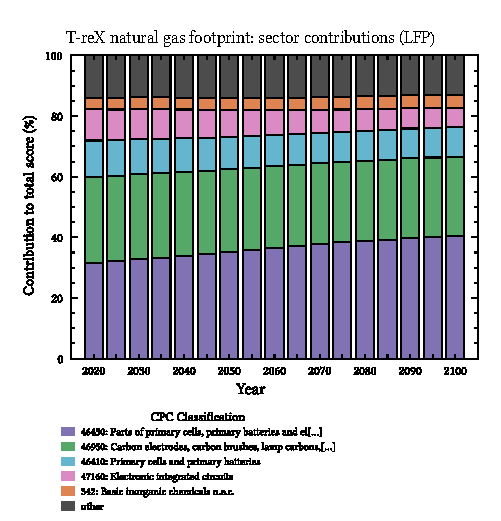
\includegraphics[width=9cm]{figures/T-reX-wastefootprint-sectorcontributions.pdf}
    \caption{Contribution of industrial sectors to the natural gas footprint of the LFP battery from 2020 to 2100 under the SSP2 scenario using the baseline RCP of the REMIND model.}\label{fig:cpc_contribution}
\end{figure}


\subsubsection{Comparison with `similar' LCIA methods}\label{sec:results-case_study-methodcomparison}

A comparison of the results from T-reX's `Coal (black)' demand method with the LCIA method `EDIP 2003 - coal no LT' is shown in~\autoref{fig:comparison_methods}. In this case, both the trends and the magnitude of the scores were very similar, both demonstrating a general decrease in the use of coking coal in the battery's footprints. Such comparability was also observed for other fossil-fuel-related methods (e.g., natural gas and petroleum), and to a lesser extent, for some of the metal demand methods (e.g., zinc and cobalt). Correlation between standard LCIA methods and T-reX methods is not generally to be expected, however, due to fundamental differences in the way that the methods are constructed. In standard LCIA methods, impact scores are derived exclusively from the magnitude of the exchanges between the biosphere and the technosphere, that is, extraction and emission. In the T-reX methods, the footprint scores are based on an accounting of either waste generated or material demand, both of which are technosphere-technosphere exchanges in terms of LCA modelling. For the material demand methods especially, this distinction is critical. For example, the application of the EDIP 2003 or the CSP methods for a given metal will provide a score that is proportional to the amount extracted by mining, whereas the T-reX method provides an aggregation of the exchanges with the market for that metal. The T-reX method, therefore, considers cases of co-production, recycling, and substitution, providing a picture of the supply chain pressures that are not captured by the standard LCIA methods. This makes the T-reX methods more sensitive to the modeling choices (e.g., economic allocation) that are generally embedded in LCA databases.

\begin{figure}[H]
    \centering
    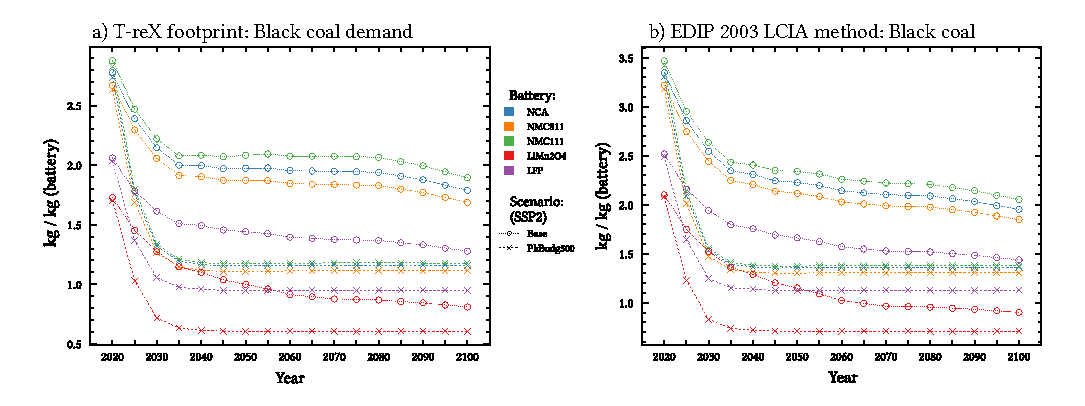
\includegraphics[width=16cm]{figures/T-reX-coalANDedip.pdf}
    \caption{Comparison of the (a) `T-reX - Coal (black)' demand footprint with the (b) conventional LCIA method `EDIP 2003 - coal no LT'  in the case study from 2020 to 2100 under the SSP2 scenario using the baseline and PkBudg500 RCPs of the REMIND model for all five batteries.}\label{fig:comparison_methods}
\end{figure}

\subsubsection{Comparison with other studies}\label{sec:results-case_study-comparison}

In the most similar published method, \cite{laurenti2023wastefootprint} used an alternative procedure for calculating the waste footprint of \~1400 activities in the \texttt{ecoinvent} database version 3.5. Direct comparison is not possible, as this database contains only one generic Li-ion battery, `market for battery, Li-ion, rechargeable, prismatic'. The inventory of this battery most closely resembles that of the NMC 111 battery in this case study. \autoref{tab:results-case_study-comparison} presents a comparison of the results from the two studies, where possible. For liquid, solid, and recycled waste, the results were closely aligned, however, for the hazardous waste fraction, Laurenti et al. reported 95\%, whereas T-reX reported only 3\%. The reason for this discrepancy is explained by the fact that in the method of Laurenti et al.\, a ``waste flow was regarded as hazardous when the hazardousness was clearly stated in its subsequent waste treatment activity''. The authors continue: ``It should be noted that the high hazardousness ratios for many products might indicate a weakness in the validity of this measure''. In T-reX, the source database is deconstructed into a list of separate exchanges, and only those explicitly defined as hazardous are marked as such.

\begin{table}[H]
    \centering
    \caption{Comparison of the results from the T-reX battery case study (database: \texttt{ecoinvent} 3.9.1 REMIND SSP2 Base 2020, activity: Li-ion NMC 111) with those from \cite{laurenti2023wastefootprint} (database: \texttt{ecoinvent} 3.5, activity:`Li-ion').}\label{tab:results-case_study-comparison}
    \begin{tabular}{lll}
        \toprule
        \textbf{Indicator}         & \textbf{T-reX} & \textbf{Laurenti et al.} \\
        \midrule
        Total solid waste (kg/kg)  & 50.9           & 62.5                     \\
        Total liquid waste (kg/kg) & 3.53           & 3.63                     \\
        Hazardous waste (kg/kg)    & 1.47           & 62.6                     \\
        Recycled waste (kg/kg)     & 1.59           & 1.98                     \\
        \bottomrule
    \end{tabular}
\end{table}



\section{Discussion}
\label{sec:discussion}
Given that both waste generation and material demand are often strongly associated with the environmental impacts of an activity, it is important that they are included in the LCA. While there are numerous examples of existing and proposed methods that attempt to provide endpoint LCIA scores through convoluted formulae or subjective weighting, there is little consensus on their application and their complexity and lack of transparency can make them difficult to use and interpret.

Our contribution advances the state-of-the-art by giving LCA practitioners a simple, flexible, and transparent way to calculate supply chain waste and material footprints, delivering results in standard units and as direct aggregations of the relevant demand inventories. Once the databases have been processed with the T-reX tool, the user can  easily apply the T-reX `pseudo-LCIA' methods to calculate the waste and material inventory footprints in the same way that they would with a conventional LCIA method.

The simple case study of five Li-ion batteries presented in this paper demonstrated the the utility, flexibility and limitations of the T-reX tool. 

First, by adjusting the user configuration for future scenarios and waste/material categorisation we easily produced a set of customised versions of the ecoinvent database. Then, by applying the T-reX `pseudo-LCIA' methods, it was trivial to calculate categorised waste and material inventory footprints for a number of present and future supply chains. Additionally, visual exploration in \texttt{ActivityBrowser} was possible because the T-reX `pseudo-LCIA' methods are integrated in the \texttt{brightway} project in the same way as standard LCIA methods.

One limitation of the T-reX tool is that it does not yet provide specific information (in a readily accessible format) on the composition of the waste generated. This is the information would be needed to thoroughly assess the potential environmental impacts of this waste. Currently, the user would need to manually explore the waste footprint inventory produced by the application of the T-reX to determine if, for example, the waste generated represents an actual loss of resources, or is simply a transfer of the `overburden' in mining activity, which is classified as `inert waste'. A methodic classification of waste exchanges and the end-of-life fates will be facilitated by the more detailed and disaggregated data that is seen in each successive release of ecoinvent~\citep{fitzgerald2023ecoinventdocumentation}.

The utility of the T-reX tool in studies of future supply chains is limited by the fact that the currently available prospective databases focus largely on changes in the energy, steel, cement, and transport sectors~\citep{sacchi2023premisedocs}. As demonstrated in the results of the case study---where there was often very little scenario-temporal change in many waste and material footprint indicators---the utility of prospective LCA is restricted if there is little adaption of the future background inventories. In particular, the inclusion of scenarios with future waste processing technology would greatly improve our predictions of waste and material flows. A strong focus on enhancing these prospective databases is, thus, of critical importance to the future of prospective LCA, and by extension, to the development of the circular economy. 

\cbox{Section word count: 450}

\section{Conclusions}
\label{sec:conclusions}
\cbox{Section word count: 250}
We have written the T-reX tool, an extension to the brightway LCA framework that enables the user to calculate the waste and material footprints of a product or service in an LCA database. It explodes the database, identifies upstream waste and material exchanges, edits them, and writes matching custom `pseudo' LCIA methods. These exchanges become pseudo-biosphere flows and thus, the footprint can be calculated as with the existing LCIA methods. The T-reX tool can be easily customised by the user to calculate the footprints of other supply-chain flows such as water, gas, and critical raw materials.

This paper extends the state of knowledge by exploring the relationship between various waste aggregation methods and environmental damage indicators, contributing to a deeper understanding of life cycle waste inventories and their association with supply-chain risk and potential environmental damage.


% Back matter
\section*{Data availability} 
All data used in this analysis are publicly available online under the noted sources. The T-reX tool is installable via the Python Package Index (PyPI) and is available at \url{https://pypi.org/project/T-reX}.
The full source code for the T-reX tool is available at \url{https://www.github.com/Stew-McD/T-reX}.
A user guide and comprehensive documentation are available at \url{https://T-reX.readthedocs.io}.

\section*{CRediT authorship contribution statement}
\cbox{Co-authors, please check this and change as necessary.}
\textbf{Stewart Charles McDowall:} Methodology, Software, Validation, Formal analysis, Investigation, Data curation, Writing - original draft, Writing - review \& editing, Visualization.
\textbf{Elizabeth Lanphear:} Conceptualization, Methodology, Software, Validation, Writing - review \& editing.
\textbf{Stefano Cucurachi:} Conceptualization, Writing - review \& editing, Supervision, Project administration, Funding acquisition.
\textbf{Carlos Felipe Blanco:} Conceptualization, Writing - review \& editing, Supervision, Project administration, Funding acquisition.

\subsection*{Alternative CRediT statement}

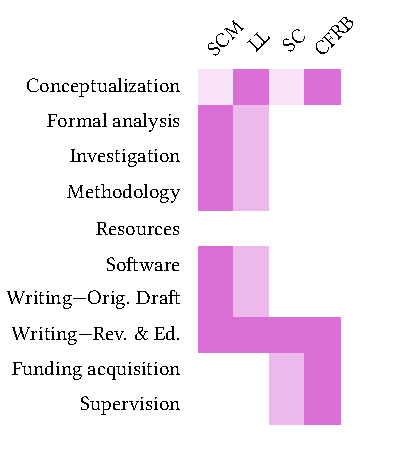
\includegraphics[width=\columnwidth, height=7cm, keepaspectratio]{credit.pdf}

\section*{Declaration of competing interest}
The authors declare that they have no known competing financial interests or personal relationships that could have appeared to influence the work reported in this paper.

\section*{Acknowledgements}
    Part of this research project was financially supported by the European Union's Horizon 2020 research and innovation programme under the grant agreement No. 101058522 (project FutuRaM --- futuram.eu). The authors would like to thank the reviewers for their valuable comments and suggestions.

\section*{Supplementary material}
    The supplementary material contains the following:
    \begin{enumerate}
        \item List of waste and material categories
        \item Example output of the T-reX tool
        \item List of identified waste and material exchanges
        \item Code (python script) used for case study
        \item Inventory and methods used in the case study
        \item Complete tabulated results of the case study
        \item Complete visualisations of the case study
    \end{enumerate}

\bibliographystyle{elsarticle-harv}
\bibliography{references.bib}
    
% \appendix


% \section{Example output}
% \label{app:example_output}

\end{document}